\section{Introduction}

%TODO: Traffic flow?
It is a well known fact that a vehicle driving at a constant velocity use less fuel than an accelerating vehicle due to the physical laws of motion\cite{Vejdir}.
In order to save fuel, one should therefore try to drive with a constant speed, but several factors prevents drivers in doing this. 
These factors are for example merging roads, blocking vehicles, traffic incidents and traffic lights. 
It is esimated that a total of 1.8 bilion Danish kroner is lost on fuel each year from all vehicles in Denmark stopping for traffic lights \cite{Vejdir}.
The socio-economic cost of time lost in traffic lights in Denmark is estimated to 9.5 billion Danish kroner. 
Lost time is defined as the delay from decelerating and stopping for a red light and the time it takes to accelerate again after\cite{Vejdir}. % In heavy congested traffic it take ekstra time for a waiting queue of vehicles to accelerrate 

Traffic lights hinders the flow of traffic as it blocks vehicles arriving from one direction in order to allow other vehicles to drive through the intersection.
Normally, a driver will only be able to guess when the light is going to change based on local knowledge of the area. 
Looking at Figure \ref{fig:Introduction:network} vehicle $\veh_2$ is approacing the intersection.
Now assume that vehicle $\veh_2$ knows the distance $\dist_3$ where he has to stop for the traffic light. 
Furthermore assume that vehicle $\veh_2$ knows that in $4$ seconds the traffic ligth will change to green. 
Then it is posible to calculate at which speed $\veh_2$ should drive such that it will drive the distance $\dist_3$ in $4$ seconds. 
Now by the time the vehicle reaches the intersection the signal will have changed and the vehicle can maintain its speed driving through the intersection.
\begin{figure}[htb]
\centering
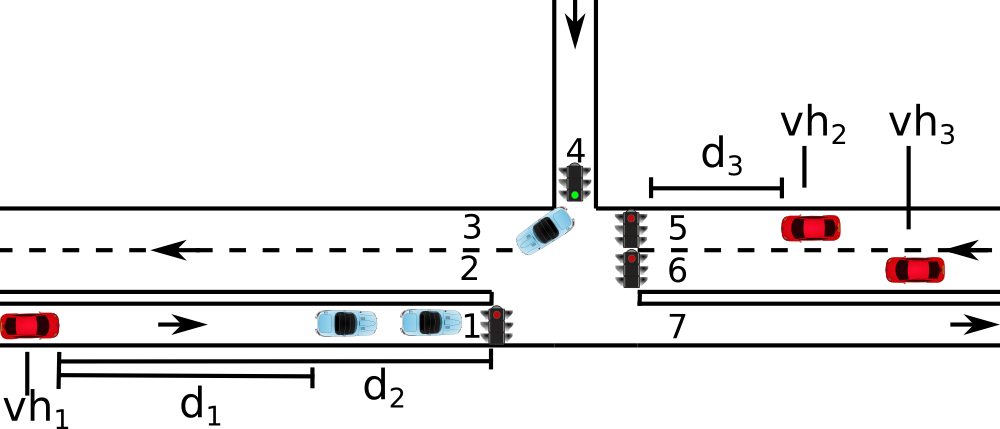
\includegraphics[width=0.45\textwidth]{../images/introNetwork.png}
\caption{Example network}
\label{fig:Introduction:network}
\end{figure}

Road authorities try to design traffic lights such that the flow of traffic is maximised in all directions.
This is very difficult, especially in junctions with changing traffic density through out the day.
Two main techniques are used for traffic lights: pretimed traffic controllers, where the signals loop between red, yellow and green in a predefined pattern; and traffic actuated controllers, where approacing vehicles are detected by road-side detectors such that the signals can be adjusted to the current traffic flow \cite{Vejdir}.
%A combination of the two is often used.
The cost of upgrading a traffic light with detectors is 200.000-300.000 Danish kroner\cite{Vejdir}.

We focus on investigating whether it is possible to reduce the fuel consumption at traffic ligths by matching driving speed to traffic lights. 
We investigate this through simulations with real-world maps, traffic data and traffic light programs. %TODO check we do this
Simulations are much cheaper, faster and safer than large-scale in-field studies. %TODO: New sentence! Does it make sense here?
We use the traffic simulator SUMO (Simulation of Urban Mobility)\cite{sumo} interfaced via TraCI (Traffic Control Interface)\cite{traci} which is a full scall microscopic traffic simulator.

We introduce the system \tech and perform realistic simmulations.
\begin{enumerate}
	\item \tech can save a considreble amount of fuel.
	\item \tech improves flow on roads with high congestion.
	\item \tech do not rely on communicaiton between vehicles and works when introducing the system to just a single vehicle.

\end{enumerate}
%TODO: Contributions?
%no communication
% system works with first vehicle
% saves fuel
% improves trafficflow
% realistic simmulation
The paper is organised as follows: 
We describe the related work in Section~\ref{sec:RelatedWork} and the model in Section~\ref{sec:Model}. 
In Section~\ref{sec:Math}, we detail the proposed techinique by going through the algorithm.
Section~\ref{sec:UseCase} is about the use case that we test the proposed technique on, and the results of these tests are evaluated in Section~\ref{sec:Test}. 
We conclude the findings in Section~\ref{sec:Conclusion}.





